% !TEX TS-program = XeLaTeX
% use the following command: 
% all document files must be coded in UTF-8
\documentclass{textolivre}
% See more information on the repository: https://github.com/leolca/textolivre

% Metadata
\begin{filecontents*}[overwrite]{article.xmpdata}
    \Title{O portal do projeto PROENEM (UNILAB) como plataforma pedagógica de ensino de argumentação e escrita}
    \Author{Adriely da Silva Clemente \sep Leonardo Chaves Ferreira \sep José Olavo da Silva Garantizado Júnior}
    \Language{pt-BR}
    \Keywords{Portal PROENEM (Unilab) \sep Recursos tecnológicos \sep Técnicas argumentativas \sep Redação estilo ENEM}
    \Journaltitle{Texto Livre}
    \Journalnumber{1983-3652}
    \Volume{14}
    \Issue{3}
    \Firstpage{1}
    \Lastpage{14}
    \Doi{10.35699/1983-3652.2021.33162}

    \setRGBcolorprofile{sRGB_IEC61966-2-1_black_scaled.icc}
            {sRGB_IEC61966-2-1_black_scaled}
            {sRGB IEC61966 v2.1 with black scaling}
            {http://www.color.org}
\end{filecontents*}


\newcounter{quote}
\newenvironment{myquote}%define new quote env
{%
\refstepcounter{quote}%
\begin{quote}(\thequote)%
}%
{\end{quote}}%

\journalname{Texto Livre}
\thevolume{14}
\thenumber{3}
\theyear{2021}
\receiveddate{\DTMdisplaydate{2021}{4}{15}{-1}} % YYYY MM DD
\accepteddate{\DTMdisplaydate{2021}{6}{1}{-1}}
\publisheddate{\DTMdisplaydate{2021}{9}{23}{-1}}
% Corresponding author
\corrauthor{Leonardo Chaves Ferreira}
% DOI
\articledoi{10.35699/1983-3652.2021.33162}
%\articleid{NNNN} % if the article ID is not the last 5 numbers of its DOI, provide it using \articleid{} commmand
% Abbreviated author list for the running footer
\runningauthor{Clemente et al.}
\sectioneditorname{Daniervelin Pereira}
\layouteditorname{Anna Izabella M. Pereira}


\title{O portal do projeto PROENEM (UNILAB) como plataforma pedagógica de ensino de argumentação e escrita}
\othertitle{The PROENEM project portal (UNILAB) as a pedagogical platform for argumentation and writing teaching}
% if there is a third language title, add here:
%\othertitle{Artikelvorlage zur Einreichung beim Texto Livre Journal}

\author[1]{Adriely da Silva Clemente \orcid{0000-0003-2537-2524.} \thanks{Email: \url{adrielyclemente@gmail.com}}}
\author[1]{Leonardo Chaves Ferreira \orcid{0000-0001-7647-4622} \thanks{Email: \url{leonardochavesferreira@gmail.com}}}
\author[2]{José Olavo da Silva Garantizado Júnior \orcid{0000-0002-9719-6366.} \thanks{Email: \url{olavogarantizado@unilab.edu.br}}}

\affil[1]{Universidade da Integração Internacional da Lusofonia Afro-Brasileira (UNILAB), Instituto de Linguagens e Literaturas, Faculdade de Letras, Acarape, Ceará, Brasil.}
\affil[2]{Universidade da Integração Internacional da Lusofonia Afro-Brasileira (UNILAB), Instituto de Linguagens e Literaturas, Programa de Pós-Graduação em Estudos da Linguagem, Acarape, Ceará, Brasil.}

\addbibresource{article.bib}
% use biber instead of bibtex
% $ biber tl-article-template

% set language of the article
\setdefaultlanguage{portuguese}
\setotherlanguage{english}

% for spanish, use:
%\setdefaultlanguage{spanish}
%\gappto\captionsspanish{\renewcommand{\tablename}{Tabla}} % use 'Tabla' instead of 'Cuadro'
%\AfterEndPreamble{\crefname{table}{tabla}{tablas}\Crefname{table}{Tabla}{Tablas}}

% for languages that use special fonts, you must provide the typeface that will be used
% \setotherlanguage{arabic}
% \newfontfamily\arabicfont[Script=Arabic]{Amiri}
% \newfontfamily\arabicfontsf[Script=Arabic]{Amiri}
% \newfontfamily\arabicfonttt[Script=Arabic]{Amiri}
%
% in the article, to add arabic text use: \textlang{arabic}{ ... }

% for russian text we also need to define fonts with support for Cyrillic script
% \usepackage{fontspec}
% \setotherlanguage{russian}
% \newfontfamily\cyrillicfont{Times New Roman}
% \newfontfamily\cyrillicfontsf{Times New Roman}[Script=Cyrillic]
% \newfontfamily\cyrillicfonttt{Times New Roman}[Script=Cyrillic]
%
% in the text use \begin{russian} ... \end{russian}

% to use emoticons in your manuscript
% https://stackoverflow.com/questions/190145/how-to-insert-emoticons-in-latex/57076064
% using font Symbola, which has full support
% the font may be downloaded at:
% https://dn-works.com/ufas/
% add to preamble:
% \newfontfamily\Symbola{Symbola}
% in the text use:
% {\Symbola }

% reference itens in a descriptive list using their labels instead of numbers
% insert the code below in the preambule:
\makeatletter
\let\orgdescriptionlabel\descriptionlabel
\renewcommand*{\descriptionlabel}[1]{%
  \let\orglabel\label
  \let\label\@gobble
  \phantomsection
  \edef\@currentlabel{#1\unskip}%
  \let\label\orglabel
  \orgdescriptionlabel{#1}%
}
\makeatother
%
% in your document, use as illustraded here:
%\begin{description}
%  \item[first\label{itm1}] this is only an example;
%  % ...  add more items
%\end{description}
 

% custom epigraph - BEGIN 
%%% https://tex.stackexchange.com/questions/193178/specific-epigraph-style
\usepackage{epigraph}
\renewcommand\textflush{flushright}
\makeatletter
\newlength\epitextskip
\pretocmd{\@epitext}{\em}{}{}
\apptocmd{\@epitext}{\em}{}{}
\patchcmd{\epigraph}{\@epitext{#1}\\}{\@epitext{#1}\\[\epitextskip]}{}{}
\makeatother
\setlength\epigraphrule{0pt}
\setlength\epitextskip{0.5ex}
\setlength\epigraphwidth{.7\textwidth}
% custom epigraph - END


% if you use multirows in a table, include the multirow package
\usepackage{multirow}

% add line numbers for submission
%\usepackage{lineno}
%\linenumbers

\begin{document}
\maketitle

\begin{polyabstract}
\begin{abstract}
O presente trabalho tem por objetivo analisar de que modo os materiais didáticos de duas oficinas, disponibilizados tecnologicamente no Portal Educacional PROENEM (Unilab), contribuíram para a construção da argumentação nos textos de estudantes pré-universitários, integrantes das ações do Projeto de Extensão Palestras Interdisciplinares e Oficinas de Produção Textual para o Enem (PROENEM). Teoricamente, nosso trabalho está alicerçado nos estudos de \textcite{perelman1996, fiorin2018} sobre as técnicas argumentativas e em \textcite{bottentuitjunior2013} sobre as características pedagógicas de um portal educacional. Foram analisadas dez redações estilo ENEM de estudantes que, ao participarem do Curso de Redação Gratuito PROENEM (Unilab), acessaram o Portal para realizar suas produções textuais.

\keywords{Portal PROENEM (Unilab) \sep Recursos tecnológicos \sep Técnicas argumentativas \sep Redação estilo ENEM}
\end{abstract}

\begin{english}
\begin{abstract}
This paper aims to analyze how the teaching materials of two workshops, technologically available on the PROENEM Educational Portal (Unilab), contributed to the construction of argumentation in the texts of pre-university students, members of the actions of the Extension Project Interdisciplinary Lectures and Textual Production Workshops for Enem (PROENEM). Theoretically, our work will be based on the studies of \textcite{perelman1996, fiorin2018} about argumentative techniques and \textcite{bottentuitjunior2013} on the pedagogical characteristics of an educational portal. Ten ENEM style essays from students who, participating in the PROENEM Free Writing Course (Unilab), accessed the Portal to make their textual productions.

\keywords{PROENEM Portal (Unilab) \sep Technological resources \sep Argumentative techniques \sep ENEM style writing}
\end{abstract}
\end{english}

% if there is another abstract, insert it here using the same scheme
\end{polyabstract}


\section{Introdução}\label{sec-intro}
O século XX possibilitou o surgimento de maneiras diferentes de adquirir informações por conta da difusão tecnológica. Recursos tecnológicos como celular, tablets e notebook fazem parte do cotidiano dos estudantes. Consequentemente, as aulas, que outrora eram completamente tradicionais\footnote{Aulas em que não há a utilização de recursos tecnológicos.}, já não são tão atrativas para os atuais alunos, sendo, portanto, necessária, sempre que possível, a integração de recursos tecnológicos para despertar o interesse dos alunos \cite{ferrari2017}.

Vale ressaltar que as tecnologias vão além de simplesmente plataformas de ambientes virtuais, pois englobam objetos de aprendizagem que proporcionam a realização do ensino a distância \cite{meirelles2017}. Além disso, os portais educacionais não contribuem apenas para os estudantes que os utilizam, mas podem auxiliar também os professores. Conforme \textcite{ferrari2017}, o professor pode integrar os recursos tecnológicos em sua prática docente como uma ferramenta apoiadora no processo de construção dos saberes, cabendo a ele apenas conhecer os novos recursos tecnológicos, adaptá-los a suas aulas e utilizá-los como apoio motivador no processo de ensino-aprendizagem. Nesse caso, o Portal Educacional PROENEM (Unilab) é uma ferramenta que, para o professor, pode possibilitar vantagens de usufruir os materiais didáticos presentes nele e utilizá-los em suas aulas de redação. 

Visando contribuir para esse despertar de interesse, o Projeto Palestras Interdisciplinares e Oficinas de Produção Textual para o Enem (PROENEM), que é uma ação social do Grupo de Pesquisa em Texto, Discurso e Ensino (TEDE) da Universidade da Integração Internacional da Lusofonia Afro-Brasileira (UNILAB), implementa, nas aulas presenciais, o uso de recursos tecnológicos como a utilização de projetor, computador e tablets. Somado a isso, o projeto também conta com o seu principal recurso, um Portal próprio que serve de suporte para propagar o conhecimento e a compreensão da importância da argumentação nos textos dissertativo-argumentativos, sobretudo nas redações estilo ENEM.

Entre os anos de 2016 a 2018, o projeto atuava exclusivamente com atividades presenciais nas escolas do Maciço de Baturité e/ou nas dependências da Unilab. No entanto, não são todos os alunos que podem participar das aulas presenciais por diversos motivos (dificuldades nos transportes, outras atividades na escola, atividades extracurriculares etc.). Por conta disso, no ano de 2019, no oferecimento do Curso de Redação Gratuito PROENEM (Unilab), o projeto passou a utilizar com mais frequência o endereço eletrônico: \url{http://proenem.unilab.edu.br/}, que é espaço oficial virtual do Portal Educacional do Projeto. Dessa forma, tornou-se possível a disponibilização gratuita de todo material elaborado pela equipe. 

As temáticas que outrora eram abordadas apenas nas escolas do Maciço de Baturité tornaram-se públicas em um ambiente abrangente a todo estudante com acesso à internet. Para conseguir alcançar cada vez mais alunos, o projeto criou uma conta oficial na rede social instagram. Por lá, as postagens, normalmente, são para divulgar alguma ação já concretizada pelos participantes do projeto e/ou para divulgar postagens novas do Portal.  Possui, na descrição dessa rede social, o link do Portal, para que, consequentemente, os internautas possam conhecer o Portal e usufruir dos materiais nele disponíveis. Deste modo, o instagram do projeto deve ser visto como um elo para direcionar os estudantes internautas ao Portal Educacional PROENEM (Unilab). 

Metodologicamente, neste trabalho, apresentaremos análises de dez redações produzidas durante duas das cinco oficinas do Curso de Redação Gratuito PROENEM (Unilab): a) “Estratégias argumentativas – comparação e exemplificação” e b) “Estratégia Argumentativa – argumentos de autoridade”. Buscamos observar de que modo os materiais didáticos das oficinas, disponibilizados tecnologicamente no Portal, os quais trabalham com os esquemas argumentativos de exemplificação, comparação e argumento de autoridade, contribuíram para a construção argumentativa nas redações estilo ENEM dos participantes.

Em termos teóricos, o presente trabalho objetiva analisar de que forma os recursos tecnológicos disponíveis no Portal Educacional PROENEM (Unilab) funcionam como ferramenta pedagógica aos estudantes que o acessam. Para isso, nos baseamos nos estudos de \textcite{bottentuitjunior2013}, sobre as características pedagógicas de um portal educacional; \textcite{iahn2001}, em seus levantamentos sobre a importância da educação virtual, e \textcite{perelman1996} sobre as técnicas argumentativas. 

Entendemos que, em muitos casos, a utilização dos recursos tecnológicos para educação, conforme \textcite{garantizadojunior2016}, possibilita o armazenamento, a distribuição e o acesso às informações independentemente do local, além de disponibilizar mecanismos pedagógicos inovadores. Examinamos neste trabalho:

\begin{enumerate}[label=(\alph*)]
\item as principais contribuições dos mecanismos tecnológicos do Portal Educacional PROENEM (Unilab), no exercício de uma interatividade importante para o processo de ensino-aprendizagem de seus usuários;
\item os impactos que os recursos do Portal Educacional PROENEM (Unilab) podem causar na construção de uma argumentação sólida, em textos estilo ENEM, dos estudantes que acessam a plataforma online.
\end{enumerate}

Em termos organizacionais, em nossa pesquisa, apresentaremos, primeiramente, o Portal em seus mecanismos tecnológicos, pautando a discussão sobre suas características pedagógicas; depois, abordaremos a relevância de recursos online de educação, ressaltando o papel do Portal no auxílio aos estudantes pré-universitários que o acessam. Por último, apresentaremos as técnicas argumentativas encontradas nas redações dos pré-universitários, ao observar o modo como os materiais das oficinas selecionadas para esta pesquisa repercutiram na construção da argumentação nos textos dissertativo-argumentativos, textos estilo ENEM.

\section{Site do PROENEM (Unilab) ou Portal Educacional PROENEM (Unilab)?}
Para que possamos entender, por exemplo, qual o motivo de chamarmos o website do Projeto de Extensão PROENEM (Unilab) de O Portal Educacional PROENEM (Unilab) e não simplesmente de Site do PROENEM (Unilab), faz-se necessário um levantamento teórico para compreendermos algumas diferenças para o uso das nomenclaturas: site e portal.
 
Acerca dessas nomenclaturas, \textcite[p. 118]{bottentuitjunior2013} assim expressa:

\begin{quote}
O termo que hoje é utilizado como portal, em meados de 1994, era conhecido como mecanismo de busca, cuja finalidade era facilitar o acesso às informações disponíveis em vários documentos dispersos pela Web. Utilizando recursos de pesquisas e navegação associativa entre hiperligações, os mecanismos de busca auxiliavam os usuários a encontrar documentos na rede. Com o objetivo de minimizar o tempo para encontrar informações relevantes na Internet e ajudar os usuários menos experientes, alguns sites de busca começaram a utilizar o conceito de portal, agrupando sites e documentos em categorias predefinidas de acordo com o seu conteúdo.
\end{quote}

Isto é, o termo portal vem sendo implementada na fala de usuários e programadores desde 1994, pois surgiu a necessidade de uma categorização mais específica e começaram a perceber que um portal possui hiperlinks, que servem para direcionar o usuário a alguma informação complementar; agrupa informações relevantes da Internet em um único local, diminuindo assim a busca em outros pontos da internet. Desse modo, o que outrora era tido apenas como “mecanismo de busca” não se encaixava mais nos padrões da época e, principalmente, na contemporaneidade, pois basta observarmos alguns comandos de busca como (Ctrl + L em documentos word e a tecla F3 em alguns computadores que serve para fazer uma pesquisa de uma dada expressão em sites da Web) para perceber que não dava mais para denominar esse tipo de site apenas chamando-o de “mecanismo de busca” e, sim, que precisaria uma terminologia que se adequasse à real função exercida.

Para a definição da palavra site, \textcite{goncalves2002} o considera como sistemas de informação, categorizando-o em oito tipos de sites com propósitos distintos uns dos outros, entre eles: 

\begin{quote}
Sites de notícias: nesta categoria, são incluídos os jornais, as revistas, os canais de rádio e TV disponíveis online; [...] Sites educativos: enquadram-se os sistemas de educação a distância, ambientes lúdico-didáticos, ambientes de ensino e aprendizagem, etc \cite[p. 115]{goncalves2002}. 
\end{quote}

Dessa forma, é possível depreender que, de maneira mais abrangente, o site contém o portal e este está contido no site Web. As categorias “de um modo geral, tentam classificar os sites quanto às suas características e utilidades. É possível ainda criar subcategorias para os sites de acordo com a sua área específica” \cite[p. 116]{bottentuitjunior2013}. Ciente disso, classificamos o Portal do Projeto de Extensão PROENEM (Unilab) não apenas como um portal informativo (por conta da aba “Notícias”), em que os internautas são informados de tudo o que ocorre no projeto de extensão, mas, sobretudo, como um ambiente virtual, ou melhor, um portal especializado na área da educação, em que estudantes e professores podem usufruir gratuitamente de materiais elaborados exclusivamente para auxiliar/aperfeiçoar a escrita de uma redação estilo ENEM. 

Destarte, entendemos e concordamos com \textcite{iahn2001} que Portais Educacionais são portais especializados na área da educação que objetivam atender às necessidades dos visitantes, tais como resolver dúvidas, propor ideias e atividades novas. Nesse sentido, o Portal Educacional PROENEM (Unilab) trabalha com três critérios propostos por \textcite{iahn2001}:

\begin{enumerate}[label=(\Alph*)]
\item Critério: atividades novas: propostas de redação – o treineiro poderá ler a ajuda ou dicas da redação a partir do tema escolhido;
\item Critérios: resolver dúvidas e propor ideias – o Portal contribui para melhorar a escrita da redação, tais como a argumentação do treineiro, do estudante. 
\end{enumerate}

Assim, a união desses critérios possibilita a formação de um “portal vertical ‘especializado em um determinado [segmento] específico’, ou seja, ‘procura atender às necessidades de um determinado grupo de usuários relacionado a um único assunto ou a uma área de interesse” (GRANDE, 2003 apud BOTTENTUI JÚNIOR, 2013, p. 120). Isto é, o Portal Educacional PROENEM (Unilab) é voltado para um ensino específico, que é o ensino de redação focalizado na temática da argumentação. Por isso, chamamos o recurso tecnológico do projeto PROENEM (UNILAB) como Portal Educacional e não simplesmente como site do PROENEM (UNILAB).

Em relação aos postulados de \textcite{bottentuitjunior2013}, sobre os portais facilitarem a busca de documento por reunir informações em um mesmo ambiente, podemos dizer que o Portal Educacional do Projeto PROENEM (Unilab) otimiza tanto o tempo dos participantes do projeto (universitários e coordenador), no sentido de procurar posteriores informações para trabalhos futuros, como também é um facilitador para participantes que desejam melhorar a argumentação na redação estilo ENEM. Isso devido ao fato de os materiais no Portal estarem agrupados em duas seções no menu vertical: \emph{Atividades Virtuais} e \emph{Atividades Presenciais}.

Essa organização do Portal “[dispõe] claramente os seus serviços e conteúdo de forma a prender a atenção de quem o estiver acessando, [...] como também [fomenta] o aprendizado e tornar-se uma ferramenta necessária para o dia-a-dia dos seus visitantes estudantes \cite[p. 67, adaptada]{iahn2001}. A seção intitulada de Atividades Virtuais, que contém em um submenu as seções “Ajuda na Redação”, “Redação Comentada”, “Podcast”, serve tanto para facilitar o uso da pesquisa quanto funciona para direcionar a atenção do estudante internauta, assim como as seções “Oficinas” e “Palestras”, que podem ser encontradas no menu vertical denominado de “Atividades Presenciais”. Ou seja, com essa organização, os estudantes podem procurar com mais facilidade qual tipo de conteúdo querem utilizar em seus estudos, porque, na categoria das Atividades Virtuais, os estudantes internautas encontrarão conteúdos desenvolvidos prioritariamente para o Portal. Na outra parte do menu vertical, os internautas encontrarão os materiais que foram utilizados nas ações dos projetos, seja nas dependências da Unilab ou em escolas do Maciço de Baturité. 

Como já dito, com o Portal Educacional PROENEM (Unilab), há a possibilidade de um acesso ao conteúdo tecnologicamente. Feito um recorte das principais informações sobre o que é um portal, passemos para as principais características do Portal Educacional PROENEM Unilab.

\section{Seções do Portal Educacional PROENEM (Unilab)}
A seguir, temos uma imagem panorâmica do Portal (\Cref{fig1}) e posteriormente um detalhamento de cada seção.

\begin{figure}[htbp]
 \centering
 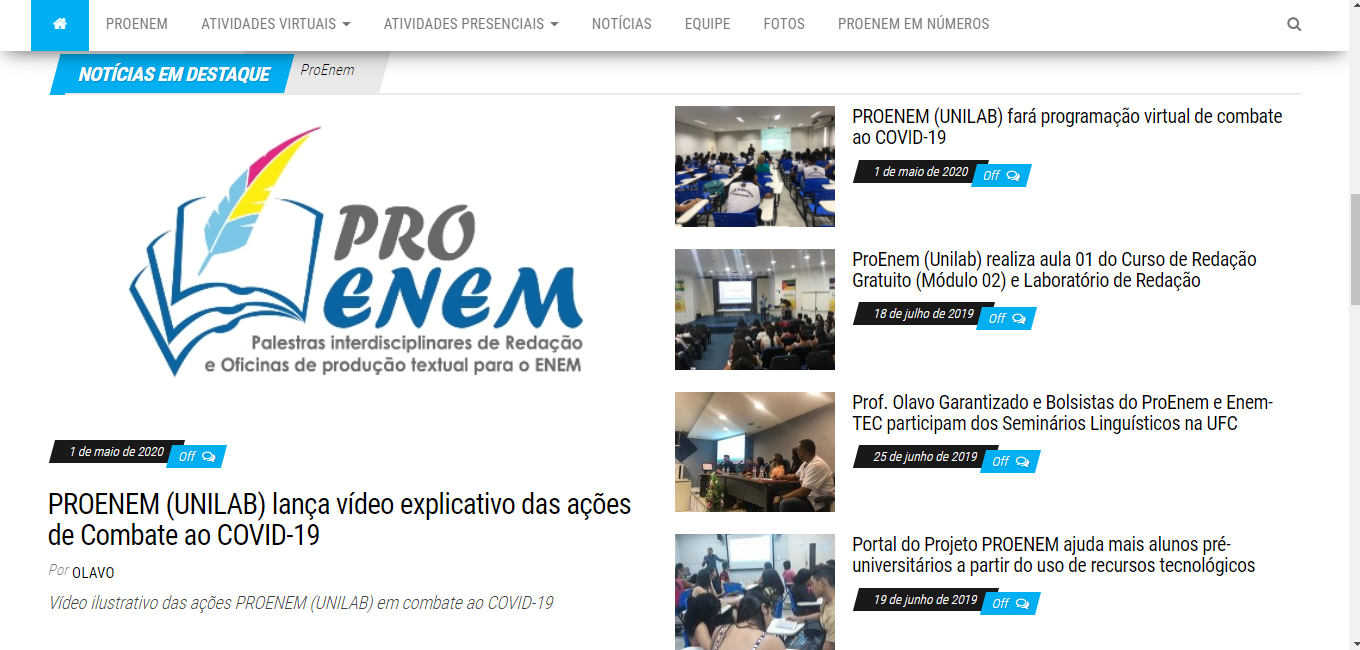
\includegraphics[width=0.8\textwidth]{fig1-33162.png}
 \caption{Portal Educacional PROENEM (Unilab)}
 \label{fig1}
 \source{www.proenem.unilab.edu.br}
\end{figure}

O Portal Educacional do Projeto de Extensão PROENEM (Unilab) possui um menu de cabeçalho fixo, em que o primeiro tópico traz a imagem de uma “casa”. Essa primeira aba apresenta uma definição sobre o que é o Projeto PROENEM (Unilab). Nele, encontra-se um vídeo lúdico com as principais informações do projeto. Podemos assim concluir que nessa aba do Portal Educacional PROENEM (Unilab) já possui os materiais digitais (vídeo, sons, animações), os quais conforme \textcite{machado2013} são:

\begin{quote}
objetos de aprendizagem [...] que tem objetivo educativo, ou seja, um embasamento pedagógico, dividido em três categorias [...]: simples: pouca interação do usuário com o objeto. Ex.: texto; intermediário: interação limitada, uma fonte de informação. Ex.: vídeo; complexo: possibilita maior interação e interatividade do usuário com o objeto. Ex.: portais \apud{machado2013}[p. 145, grifo nosso]{meirelles2017}.
\end{quote}

Ainda nessa primeira parte o Portal Educacional PROENEM (Unilab) possui a seção intitulada “Notícias em Destaque”, que indica as principais notícias que ocorreram recentemente no projeto, estabelecendo, portanto, atualização informacional dos principais acontecimentos das ações do projeto de extensão. Ainda na primeira seção, na mesma página, o Portal apresenta um espaço reservado para os sites oficiais do ENEM, intitulada “Sites Importantes”, que direciona o internauta, caso este clique nos hiperlinks das imagens, para os sites do Instituto Nacional de Estudos e Pesquisas Educacionais Anísio Teixeira (INEP) e do INEP Enem, em que ele poderá se informar dos cronogramas oficiais do Exame Nacional do Ensino Médio.

O menu de cabeçalho fixo do Portal Educacional PROENEM (Unilab) possui também as seguintes opções: 

\textbf{PROENEM:} apresenta a descrição do projeto, tais como o histórico, metodologia utilizada nas atividades e a base teórica do projeto. Há a presença, também, em forma de textos e imagens, das “Atividades do PROENEM UNILAB”, tais como o “Curso de Redação Gratuito na Unilab”, “Oficinas interdisciplinares”, “Palestras interdisciplinares”, “Laboratório de Redação Gratuito” e “PROENEM Social’. Encontra-se, ainda, a descrição de quem é o “Público-Alvo do projeto”.

\textbf{ATIVIDADES VIRTUAIS:} engloba conteúdos elaborados prioritariamente para o Portal. É dividido com um submenu vertical com os seguintes tópicos:

\begin{itemize}
\item \emph{Podcast}: ambiente que conta com o desenvolvimento de dez episódios de podcasts. São eles: “A redação no ENEM”; “A dissertação-argumentativa; Critérios da prova de redação do ENEM”; “Uso dos textos motivadores”; “Textos multimodais e construção da argumentação na redação”; “Estrutura da redação estilo ENEM (introdução; parágrafos de desenvolvimento; parágrafo de conclusão)”; “Técnicas argumentativas na redação estilo ENEM” e “Conectivos e construção da argumentação”. Nesta aba, os estudantes podem ouvir os conteúdos sobre redação. 
\item \emph{Vídeo-Aulas}: gravações de aulas ministradas pelo Prof. Dr. Olavo Garantizado, coordenador do projeto, sobre a redação estilo ENEM;
\item \emph{Proposta de redação}: local em que são disponibilizadas as propostas de redações para download, além de textos explicativos para cada tema.
\item \emph{Ajuda na redação}: com um submenu com as seguintes opções: \emph{Propostas de Redações Comentadas}, onde os integrantes do projeto comentam por meio de texto, quais os pontos, de acordo com o tema/proposta da redação, os estudantes poderão abordar na produção textual. Ao fazer isso, o projeto PROENEM (Unilab) utiliza o recurso tecnológico, Portal Educacional PROENEM (Unilab), como um instrumento para colaborar com a aprendizagem do aluno, pois, lendo a ajuda sobre o tema, o estudante compreenderá melhor a proposta; Envie sua redação, que contém um formulário onde os internautas podem enviar um arquivo para os corretores do PROENEM corrigirem, para que estes, posteriormente, possam enviar por e-mail a nota, explicação da redação para o participante e \emph{Dicas de Redação}.
\end{itemize}

Na seção “Envie sua redação”, a interatividade da página web possui um formulário para escrever e enviar o texto da redação. Consequentemente, o usuário receberá uma resposta automática. Essa resposta automática é enviada para o e-mail do aluno, informando-o que em até sete dias receberá a redação corrigida. Por consequência, essa possibilidade de correção online diminui o gasto com papéis e, caso seja utilizada por professores do ensino básico, por exemplo, otimizará até o tempo de correção dos textos dos alunos, pois quem faria a correção das redações seriam os corretores do PROENEM (Unilab) e não necessariamente o docente da escola. Se for utilizada pelo estudante, funciona como a possibilidade de treinar/aperfeiçoar a escrita da redação.

Na seção “Dicas de Redação”, há “a interdisciplinaridade, tão em voga neste século no âmbito educacional, [...] trabalhada de maneira prática, [...] oportunizando a interação entre diversas áreas do conhecimento” \cite[p. 39]{ferrari2017}. Ou seja, é o ambiente que apresenta informações adicionais para a escrita da redação estilo ENEM, tais como explanações de como o estudante pode aumentar a nota a partir das cinco competências exigidas na redação do Exame, como utilizar autores das Ciências Humanas para contribuir com o avanço na argumentação escrita, entre outras dicas;

\textbf{ATIVIDADES PRESENCIAIS:} expõe os conteúdos que foram utilizados nas ações presenciais do projeto. É dividido em um submenu vertical com os seguintes tópicos:

\begin{itemize}
\item Oficinas: é publicado um breve resumo e as principais fotos do dia de cada oficina ministrada presencialmente. Assim, os internautas podem ficar informados sobre o que ocorreu durante o período de cada aula.
\item Palestras: seção parecida com a aba “Notícias”; porém, nesta, propagam-se as palestras extras e as que são abertas para a comunidade externa. Essas pessoas, posteriormente, poderão ser beneficiadas com a arrecadação de alimentos promovida pela ação beneficente do Projeto.
\item Cursos: possui um submenu vertical com as seguintes seções: Editais – local onde se agrupam os comunicados de seleção para graduandos da Unilab atuarem como voluntários no projeto. Curso de Redação – aborda as principais informações para os matriculados nos cursos gratuitos promovidos pelo projeto de extensão, bem como a disponibilização dos materiais para quem não pode\footnote{Referimo-nos essencialmente àquelas pessoas que não conseguiram a vaga, pois ela é limitada, assim como também àqueles para os quais o horário se torna inacessível.} participar do curso e/ou para revisão das aulas, ou seja, tanto o estudante matriculado no curso poderá estudar em sua própria residência ou em outros ambientes com mais liberdade e flexibilidade de horários quanto os visitantes do Portal, pois, de acordo com “[...] especialistas em Tecnologias Educacionais [...] não importa o dispositivo utilizado (celular, \emph{tablet} ou computador), mas ‘como está sendo feita a mediação entre a informação e o que o aluno está fazendo’” \cite[p. 153]{meirelles2017}. No caso, o ensino não será tão diferente para aqueles que estavam na aula presencial do que para aqueles que não estavam presentes, pois “a mudança na dinâmica da aula presencial, [...] gera mais liberdade e flexibilidade, mas, por outro lado, exige do aluno responsabilidade com prazos e resultados, o que exige também senso crítico” \cite[p. 162]{meirelles2017}. Nessa seção, “Curso de Redação”, por sua vez, é dividida nos subitens: \emph{Módulos} – em que apresenta o cronograma de cada curso, bem como a descrição do assunto abordado pelos palestrantes e os materiais de cada aula. Os conteúdos são anexados sempre após o término da aula presencial. \emph{Materiais usados} – é a parte onde os materiais em PDF do curso e das palestras ficam mais organizados para o acesso, e a seção \emph{Inscrições} é onde o internauta é direcionado para o endereço eletrônico: \url{https://www.even3.com.br/cursoderedacaoproenemmoduloii2019/} para poder matricular-se apenas em um ou em todas as ofertas disponíveis para o curso, tais como: participar de laboratório de redação e/ou palestras e/ou oficinas. Ainda no submenu “Cursos”, há a opção: \emph{Corretores de redação} – onde há os subitens: \emph{Inscrições e Módulos Básico (20 horas)}, em que aquele apresenta um formulário para os possíveis interessados em tornarem-se voluntários do projeto de extensão e/ou apenas para adquirirem horas complementares exigidas pela Instituição Unilab e esse apresenta o que será tratado no módulo básico de 20 horas. Em outras palavras, o submenu “Cursos” é a parte do Portal voltada preferencialmente para o público acadêmico.
\end{itemize}

\textbf{NOTÍCIAS:} informatização para os internautas sobre o que acontece e acontecerá no projeto de extensão (online e/ou offline).

\textbf{EQUIPE:} parte do menu que apresenta o nome e as funções que os integrantes exercem no projeto de extensão.

\textbf{FOTOS:} parte do menu que reúne os registros fotográficos das ações realizadas no projeto.

\textbf{PROENEM EM NÚMEROS:} local que agrupa alguns dos principais números do projeto desde o ano de 2016. Nessa parte, existe a possibilidade de internautas deixarem algum comentário/resposta sobre o que desejarem e pode haver algum bate-papo.

Como observamos, o Portal Educacional PROENEM (Unilab) conta com uma gama de recursos tecnológicos interativos. Esses recursos facilitam tanto a sua utilização quanto possibilitam uma aprendizagem online mais interativa, por parte dos estudantes que usam o Portal. Desse modo, passaremos agora à investigação dos impactos que os recursos do Portal Educacional PROENEM (Unilab) podem causar na construção de uma argumentação sólida, em textos estilo ENEM, dos estudantes que acessam a plataforma online.

\section{O Portal Educacional PROENEM (Unilab) como instrumento pedagógico de construção da argumentação}
Cada usuário com acesso à internet desfrutará, gratuitamente, dos conteúdos disponibilizados no Portal Educacional PROENEM (Unilab). Em relação à contribuição do Portal com a argumentação das redações, no que se refere à disponibilidade dessas ferramentas pedagógicas, é possível notar que há materiais voltados e desenvolvidos para a temática (textos de dicas de redação, materiais das oficinas, podcast, entre outros).

Nesses materiais, o objetivo é fazer com que os pré-universitários compreendam \emph{o que é}, \emph{para que serve} e \emph{como utilizar as técnicas argumentativas} na escrita durante as redações. Consequentemente, de maneira didática e prática, eles poderão compreender o que \textcite{perelman1996} dizem sobre o objetivo da argumentação na adesão à tese apresentada, ou seja, os internautas e participante do PROENEM (Unilab), candidatos ao ENEM, entenderão que não devem apenas parafrasear os textos motivadores, mas sim argumentar para defender um ponto de vista convincente ao corretor. 

\textcite{perelman1996} reconhecem a dificuldade que o orador pode encontrar em tentar definir o seu auditório, sobretudo no que diz respeito a um escritor, pois este não sabe quem serão seus leitores. No entanto, ao adaptar esse comentário para os textos estilo ENEM, o auditório seria o corretor do ENEM, pois nesse exame o vestibulando, ao escrever seu texto dissertativo-argumentativo, deve persuadir o corretor da redação, porque o texto é “avaliado por, pelo menos, dois professores, de forma independente, sem que um conheça a nota atribuída pelo outro” \cite[p. 6]{inep2019}. Isso já facilita também a escrita, porque Irandé \textcite{antunes2003} diz que o aluno precisa entender o que e para quem está escrevendo. Ciente de quem corrigirá a prova da redação, o estudante poderá ficar mais tranquilo nesse aspecto. Porém, precisa entender e compreender que o texto é:

\begin{quote}
Em prosa, do tipo dissertativo-argumentativo, [...] [precisa] defender uma tese – uma opinião a respeito do tema proposto –, apoiada em argumentos consistentes, estruturados com coerência e coesão, formando uma unidade textual [...] redigido de acordo com a modalidade escrita formal da língua portuguesa [...] elaborar uma proposta de intervenção social para o problema apresentado no desenvolvimento do texto que respeite os direitos humanos \cite[p. 5, adaptada]{inep2019}.
\end{quote}

Desse modo, como a redação deve ser escrita no formato dissertativo-argumentativo, o participante deverá descrever o assunto e "apresentar razões que justificam ou refutam um determinado ponto de vista" \cite[p. 223]{fiorin2018}, ou seja, argumentar, apresentar uma proposta de intervenção para finalizar o texto. Os critérios de avaliação da redação do ENEM, além de serem descritos detalhadamente na Cartilha do Participante para a redação do ENEM, são abordados também no Portal Educacional PROENEM (Unilab). São trabalhados na seção \emph{Dicas de Redação}. Entre as dicas podemos citar: \emph{Compreendendo a avaliação da competência II} e \emph{Critérios da prova de redação do ENEM}, assim como, no Portal, há a possibilidade de discentes acadêmicos matricularem-se no curso de corretores para conhecer e aprender o modo de correção estilo ENEM.

Nesse sentido, ao observar, por exemplo, dois dos cinco materiais utilizados no primeiro módulo do Curso de Redação Gratuito PROENEM (Unilab), o internauta aprenderá a focar em pelo menos três esquemas argumentativos apresentados por \textcite{perelman1996} – argumento pelo exemplo, argumento por comparação e argumento de autoridade.

O argumento pelo \emph{recurso ao exemplo} é uma estratégia argumentativa baseada na estrutura do real. Desse modo, esse argumento se caracteriza pela presença de argumentos que recorrem ao caso particular, ou seja, há uma generalização de ocorrências a partir de casos particulares. Assim, conforme \textcite{perelman1996}, em argumentos que recorrem ao mecanismo da exemplificação, o locutor tenta apresentar o exemplo particular com o objetivo de estabelecer no auditório certas conclusões. É nesse ponto que o argumento pelo exemplo, conforme \textcite[p. 197]{garantizadojunior2015}, enfatiza, busca generalizar baseando-se em casos particulares.

Já a outra técnica argumentativa abordada nos materiais disponíveis no Portal é a comparação. Essa estratégia está inserida dentro do que \textcite{perelman1996} chamam de “argumentos quase-lógicos”. Isso quer dizer que as estratégias envolvidas nesse tipo de argumento possuem sua força argumentativa a partir de juízos preferíveis em que a conclusão é “provável, possível, plausível, mas não logicamente necessária” \cite[p. 115]{fiorin2018}. De forma geral, os argumentos construídos por recursos comparativos estão ligados a um efeito de avaliação, de A em relação B. Desse modo, esses argumentos têm um objetivo do autor, em relacionar objetos com uma ideia de mediação que pode reforçar tanto uma desigualdade quanto uma igualdade. Segundo \textcite[p. 291]{perelman1996}, esses modos de avaliação, advindos das comparações, podem ocorrer por oposição, por ordenamento e por ordenação quantitativa.

Por sua vez, o argumento de autoridade, também presente no componente didático no Portal, entre as redações, pode vir a se apresentar por meio de citações diretas e indiretas. Assim, o estudante sustenta o seu ponto de vista a partir do discurso de um pensador e/ou escritor renomado em torno do tema. Ao falar dessa estratégia argumentativa, \textcite{menezess2011} salienta: “o mais característico argumento de prestígio é o argumento por autoridade” \cite[p. 50]{menezess2011}, isso porque certos juízos de um insigne orador acabam funcionando como um bom argumento a favor de uma tese.

É importante frisarmos que essas estratégias são básicas e cruciais quando falamos em textos dissertativo-argumentativos estilo ENEM. Elas estão inseridas dentro de competências, exigida pelo Exame, quanto à organização das informações para o desenvolvimento da argumentação no texto. Na competência III, o corretor deve avaliar a seleção, relação, organização e interpretação de informações, fatos e opiniões em defesa de um ponto de vista. Desse modo, essa competência avalia a qualidade e consistência argumentativa, levando em conta a capacidade de persuasão do autor do texto por meio dos recursos argumentativos que ele utiliza, seja uma comparação, um exemplo ou a citação de alguma autoridade.

Como dito anteriormente, no oferecimento desses materiais no Portal, o projeto busca fazer com que os pré-universitários compreendam \emph{o que é}, \emph{para que serve} e \emph{como utilizar as técnicas argumentativas} na escrita durante as redações. Para isso, são disponibilizados, gratuitamente online, os materiais didáticos que foram utilizados para esta pesquisa.

Esses materiais estão divididos em dois tópicos distintos: “Estratégias argumentativas – comparação e exemplificação” e “Estratégia Argumentativa – argumentos de autoridade”. Apesar disso, a estrutura pedagógica dos materiais se apresenta de modo muito homogêneo e isso se deve ao fato dos materiais terem sido produzidos em conjunto nos estudos do Grupo de Pesquisa em Texto Discurso e Ensino (TEDE/UNILAB).

Dessa forma, a produção no material a ser disponibilizado no Portal se pautou em três pontos: (i) apresentação inicial, (ii) construção argumentativa e (iii) Prática. Essa organização se deve ao fato de, ao longo dos estudos e das diversas análises feitas pelo Grupo TEDE/Unilab no que se refere às redações pré-vestibulares, termos percebido a dificuldade dos estudantes na adequação ao caráter argumentativo do tipo de texto exigido pelo ENEM.

Então, no primeiro ponto, apresentação e discussão, o material busca oferecer aos alunos algumas informações necessárias para que eles identifiquem melhor a estratégia argumentativa que é repassada. Nesse sentido, o cerne inicial do material recai sobre perguntas e respostas que mostram a relevância desse tipo de conteúdo para redações estilo ENEM: Que argumento é esse? Quais competências exigidas ele atinge? Que forma ele assume durante a escrita do texto? Como podemos praticá-lo? Essa “apresentação inicial”, presente nos materiais disponíveis no Portal, funciona como um mecanismo pedagógico que busca tornar a aprendizagem mais educativa e eficiente.

O segundo ponto é o da “construção argumentativa”. Essa seção dos materiais contribui para um contato mais direto com as estratégias argumentativas trabalhadas e, desse modo, são apresentados alguns exemplos que indicam como os tipos de argumentos se estruturam dentro de textos estilo ENEM. É destacado, portanto, como determinados argumentos se configuram nos textos dissertativos-argumentativos, seja por meio de recursos referenciais, marcas linguísticas de coesão e, até, no caso do argumento por autoridade, com o uso de citações diretas e indiretas. Dessa forma, apresentados os mais variados exemplos, busca-se deixar os estudantes mais cientes e preparados quanto à organização de determinados argumentos ao longo de suas produções.

O terceiro ponto é o momento da “prática” e nele são oferecidos aos alunos temas propícios para a construção dos argumentos apresentados nos tópicos. No caso dos argumentos por comparação e exemplificação, temos o tema “Caminhos para o combate à violência contra criança”. Dessa forma, para que a argumentação aconteça de modo plausível, o material oferece diversas informações e estatísticas que podem ser utilizadas para o desenvolvimento de argumentos comparativos e exemplificativos nos textos dos estudantes. Não diferente disso, no caso do tópico sobre os argumentos de autoridade, o tema é “Violência nas escolas do Brasil: \emph{bullying} e suas consequências”. Para que os alunos possam utilizar argumentos baseados em autoridades sobre o assunto, o material oferece a explicação e exemplificação de citações selecionadas para o tema, dentre os estudiosos da educação.

À vista disso, conseguimos depreender que recursos tecnológicos como os oferecidos pelo Portal, adotando uma organização didática, são ferramentas pedagógicas eficazes para o ensino. É nesse sentido que pretendemos mostrar os recursos tecnológicos do Portal Educacional PROENEM (Unilab) como uma ferramenta pedagógica, voltada para o trabalho com redações de estudantes pré-universitários, para a construção da argumentação em textos dissertativo-argumentativos estilo ENEM. 

Dessa forma, buscando mostrar os impactos que os recursos do Portal Educacional PROENEM (Unilab) podem causar na construção de uma argumentação sólida, em textos estilo ENEM, dos estudantes que acessam a plataforma online, passaremos na próxima seção à análise das redações que foram produzidas durante duas oficinas (já mencionadas) do curso de redação gratuito no projeto. 

\section{Análise das técnicas argumentativas: redações do módulo 1 do Curso de redação gratuito PROENEM (Unilab)}
"Não podemos esquecer-nos que a palavra \emph{argumento} é formada com a raiz argu-, que significa ‘fazer brilhar, cintilar’ [...] o argumento é o que realça, o que faz brilhar uma ideia” \cite[p. 22]{fiorin2018}. Ao trazer para o contexto as redações dos estudantes, o que chama mais atenção nos textos estilo ENEM é o modo como eles utilizam as palavras, organizam as ideias nas redações: “Caminhos para o combate à violência contra criança” e “Violência nas escolas do Brasil: \emph{bullying} e suas consequências” para persuadir o corretor. 

Sendo assim, como a estrutura solicitada é o texto dissertativo argumentativo, o estudante precisará, além de falar sobre o assunto, defendê-lo por meio da utilização adequada dos argumentos, pois como "um argumento é uma razão a favor ou contra um determinado ponto de vista [...] deve ser pertinente ao tema que está em debate." \cite[p. 176]{fiorin2018}. Diante disso, os exemplos a seguir apresentam as estratégias argumentativas encontradas nas redações, que foram solicitadas no primeiro módulo do Curso de Redação Gratuito do PROENEM (Unilab). Optamos por apresentar a originalidade do texto escrito dos pré-universitários sem as correções ortográficas, porque nosso foco, nesta parte da pesquisa, é analisar as técnicas argumentativas presentes nas redações.

Dessa forma, observamos nos textos uma diversidade de argumentos já postulados na abordagem teórica da Nova Retórica de Perelman e Olbrechts-Tyteca. Um exemplo disso é o argumento por comparação. Esse tipo de argumento, segundo \textcite[p. 291]{perelman1996}, tem um objetivo do autor, em relacionar objetos com uma ideia de mediação que pode reforçar tanto uma desigualdade quanto uma igualdade. Vejamos o seguinte trecho:

\begin{myquote}\label{quote1}
“O trabalho infantil está presente na sociedade brasileira há muito tempo. Dessarte como diversos outros tipos de exploração contra jovens. Assim como à revolução industrial explorou moçoilos nas primeiras indústrias por conta da mão de obra barata, que quase sempre eram crianças abandonadas em orfanatos”. (RED02-TURMA1).
\end{myquote}

Em (\ref{quote1}), o Locutor inicia com a afirmativa de que o trabalho infantil está presente na sociedade há tempos. Para justificar essa assertiva, ele compara que a Revolução Industrial, durante o século XVII e XIX, já utilizava a exploração dos mais jovens. Faz, portanto, o uso da técnica argumentativa de comparação. A comparação feita foi entre épocas diferentes (o século referente ao momento da Revolução Industrial para a atualidade) que consequentemente possui a comparação entre lugares distintos (Europa X Brasil), aproximando duas realidades distintas com objetivos argumentativos. 

Vejamos mais outros dois exemplos com a mesma estratégia argumentativa:

\begin{myquote}\label{quote2}
"Na série de tv americana 'Os 13 porquês' é retratado a vida e a morte de Hanna meu Baker, que quando se suicida deixa 13 fitas em que cada uma delas é contando um motivo que à levou à cometer tal ato. Com o passar dos episódios é descoberto que um dos maiores motivos que fez com que Hanna tirasse sua vida foi o bullying. Infelizmente o que é retratado na série não é algo longe da vida real." (REDLB201905).
\end{myquote}

\begin{myquote}\label{quote3}
“A 30, 50 anos atras um pai ou uma mãe bater no seu filho era normal, assim, como nas escolas usarem palmatórias, deixarem as crianças de joelho em cima de grãos, crianças não estudarem só trabalharem, [...] Hoje existe um orgão que é por lei para proteção da criança e do adolescente O conselho tutelar que protege contra abuso, e qualquer tipo de violência e fiscaliza a vida estudantil, entretanto existem falhas na atuação do concelho, não é rigoroso. Compreendo que para realmente funcionar, teria que ser com profissionais realmente qualificados, [...]”. (RED05-TURMA1).
\end{myquote}

Em (\ref{quote2}), o Locutor utiliza a narração para contextualizar a série Os 13 porquês. Ao fazer isso, primeiramente está de acordo com o que o Manual do Candidato ao Enem denomina "pequenas narrações ilustrativas". Desse modo, ele utiliza a técnica argumentativa da comparação para fazer uma relação com o caso do bullying da série com o que acontece infelizmente na realidade. 

Já em (\ref{quote3}), para além da comparação, temos a presença de outro recurso argumentativo: a exemplificação. Primeiramente, ao abordar a noção da palmatória, que vogava no século XIX, o Locutor sugere um confronto entre épocas distintas, pois a criação do Estatuto da Criança e do Adolescente foi em 1990 e a palmatória tornou-se crime no Brasil em 1980. Dessa forma, há uma noção de comparação nesse trecho da redação estilo ENEM. Ao dizer que o Conselho Tutelar protege “qualquer tipo de violência” e a palmatória é um grau de violência, o vestibulando utiliza esse recurso comparatístico para afirmar que outrora a palmatória era “legal” e após a criação do Conselho ela torna-se ilegal em crianças. Fato este que desde 1970 foi repensado através de campanhas pelo fim da violência infantil, ou seja, compara que anos atrás acontecia esse ato e que na atualidade não ocorre mais. 

Além disso, a estratégia da exemplificação também se realiza em (\ref{quote3}). Isso porque, no texto, o estudante apresenta algumas formas consideradas por ele um ato de violentar uma criança. Entre eles está a palmatória, o ato de ajoelhar-se em cima de grãos, o direito ao estudo banido e sendo imposto o dever de trabalhar. Fazendo isso, ele utiliza a estratégia perelmaniana da exemplificação para fundamentar sua tese. Primeiramente, ele apresenta alguns exemplos de violência e, logo após, argumenta que o Conselho Tutelar não atua de maneira rígida nesses aspectos. Sugere que, para o funcionamento do Conselho, este deveria ter “profissionais realmente qualificados” para atuar na área e ser a favor do direito infantil contra as violações, isto é, apresenta exemplos reais de pessoas que sejam qualificadas para trabalhar com a idade do público infanto-juvenil.  

Desse modo, o argumento pelo exemplo chama, para dentro da tese defendida, um exemplo que lhe fundamente. Esse recurso argumentativo se fez presente também nos seguintes trechos:

\begin{myquote}\label{quote4}
“A nova legislação traz alguns avanços e bons projetos para combater a violência contra as crianças e adolescentes como campanha de conscientização periodicamente para conscientizar a população na indentificação de violências contra crianças. E a criação de atendimento telefonico para denúncias de violência, apesar de ser uma boa legislação ainda podemos fazer algo mais. Diante dessa perspectiva, cabe avaliar os fatores que favorecem esse quadro”. (RED03-TURMA1).
\end{myquote}
\begin{myquote}\label{quote5}
“O abuso sexual é uma das violências contra crianças mais comum, na maioria dos casos, a vítima conhece o agressor, que as vezes é alguém da própria família. O abusador ameaça a vítima, que com medo, não denuncia o abuso sofrido” (RED03-TURMA3).
\end{myquote}

No exemplo (\ref{quote4}), o Locutor apresenta em seu parágrafo de redação dois exemplos de projetos que a nova legislação utiliza contra a violência infantil: as campanhas de conscientização e o atendimento telefônico como possíveis formas de combater a violação do direito da criança. Para isso, o pré-universitário argumenta que, apesar de existir essas ações, a nova legislação ainda precisa melhorar e rever pontos que apenas na teoria não funcionam. Ou seja, como a técnica perelmaniana de exemplificação é enquadrada nos argumentos baseados na estrutura do real, o aluno utiliza essa técnica para mostrar que, apesar dos projetos reais da Legislação existirem, ainda ocorre a violência infantil. Em (\ref{quote5}), há também o uso da estratégia por exemplificação, pois o estudante apresenta que o abuso sexual é um dos exemplos de violação provocados pelo agressor na criança e que muitas vezes é alguém da própria família que abusa. 

Outro tipo de argumento presente em nossas considerações, com base nos achados de \textcite{perelman1996, fiorin2018}, é o recurso a uma autoridade. Essa estratégia consiste, segundo os autores da \emph{Nova Retórica}, em relações de prestígio, na utilização de juízos de outras pessoas como forma de provar uma tese. Um exemplo dessa técnica se mostrou evidente no exemplo a seguir:

\begin{myquote}\label{quote6}
“De acordo com Artigo 3 da Declaração Universal dos Direitos Humanos promulgada em 1948 pela ONU (Organização das Nações Unidas, - todo ser humano tem direito à vida, à liberdade e à segurança pessoal. No entanto, a incidência de violência contra crianças, impede que isso aconteça na prática”. (RED04-TURMA3).
\end{myquote}

Em (\ref{quote6}), o Locutor baseia-se no argumento de autoridade para fundamentar sua tese. Essa técnica é encontrada no momento em que cita o artigo III da Declaração Universal dos Direitos Humanos, pois, como o artigo diz que todo ser humano tem o direito à vida, à liberdade e à segurança pessoal e a criança é um ser humano, elas possuem esse direito (princípio lógico). No entanto, o estudante afirma que, na prática, esse direito está sendo violado. Ou seja, ao citar o decreto que protege todo ser humano, o vestibulando respalda-se na autoridade da lei para persuadir o corretor. Essa mesma técnica argumentativa, podemos encontrar no exemplo seguinte:

\begin{myquote}\label{quote7}
“Psicólogos afirmam o que na maioria das causas do suicídio, o bullying tem grande participação, fazendo com que a vítima desenvolver problemas emocionais, alguns chegam ou chegaram a ser espancados até perder a consciência por motivos que nem o mesmo, consegue entender o porquê. as escolas precisam dar mais atenção são, trabalhar o tema em sala e promover debates.” (REDLB201918).
\end{myquote}

No exemplo (\ref{quote7}), podemos constatar que o Locutor usa o mesmo tipo de argumento, mas de um modo mais peculiar. Nesse caso específico, não temos citações direta ou indireta de algum pensador, mas é salutar observar uma relação de prestígio estabelecida a um determinado perfil profissional. Nesse sentido, para justificar que o bullying gera problemas emocionais nas vítimas, o estudante recorre a uma afirmação feita por especialistas no estudo do comportamento e das funções mentais, os psicólogos.

Outro tipo de argumento encontrado em nosso corpus consiste na valorização dada a um determinado acontecimento de acordo com as suas consequências. Essa técnica argumentativa pode ser observada no seguinte exemplo:

\begin{myquote}\label{quote8}
“Muitas das vezes, as pessoas que sofrem com o bullying desenvolvem depressão após serem rejeitadas diariamente por uma ou um grupo de pessoas, logo se excluem da sociedade por achar que exista algum problema com elas mesmas, se auto culpabilizam pelo que passam, e em consequência, a depressão resulta em suicídio em muitos casos." (REDLB201905).
\end{myquote}

Em (\ref{quote8}), é possível notar que o pré-universitário apresenta consequências que o bullying causa na vida do atacado: isolamento, culpabilidade e depressão, e esta leva ao suicídio, ou seja, utiliza a técnica argumentativa nomeada por \textcite{perelman1996} de \emph{O vínculo causal como relação de um fato com sua consequência}, isto é, apresenta e justifica que a consequência de sofrer bullying gera a depressão, e esta é um dos meios para levar ao suicídio. Esse tipo de argumento também foi verificado em outras redações, como em:

\begin{myquote}\label{quote9}
“[...] Outro grave problema dentro da sociedade é o abandono dos estudos por parte dos jovens, que por estarem sujeitos a agressões acaba por desacreditar de um futuro melhor proporcionado pelos estudos, o que o deixa propicio a ser marginalizado pela sociedade [...]”. (RED02-TURMA1).
\end{myquote}

No exemplo (\ref{quote9}), o pré-universitário sustenta a tese de que o abandono escolar, como consequência de condições sociais desfavoráveis, existe por causas maiores, como a negligência, o abandono e o trabalho infantil. Nessa estratégia, o vestibulando explicita um acontecimento, que é o abandono dos estudos, e a existência de uma causa que pode determiná-lo, no caso, a violência e a negligência, expressando um dos modos pelos quais esse tipo de argumento pode se externar.

Uma outra técnica argumentativa encontrada em nosso \emph{corpus} consiste em um esquema tido como quase-lógico por \textcite{perelman1996}. O argumento por probabilidade. Pode ser considerada uma das técnicas mais “fáceis” de serem identificadas, porque ela utiliza dados numéricos para respaldar uma dada opinião. Para entender melhor, observemos o trecho:

\begin{myquote}\label{quote10}
“[...] o número de violência contra crianças tem crescido muito nos dias de hoje [...] existem várias denúncias, mas de nada adianta, pois o número só aumenta. Porcentagem de denúncias passada pelo disque 100, negligência (73,07\%), psicológica (47,07\%), sexual (24,19\%).” (RED04-TURMA1).
\end{myquote}

Em (\ref{quote10}), para comprovar a tese de que a violência contra a criança tem um índice alarmante nos dias atuais, o pré-universitário apresenta dados estáticos para comprovar que, apesar de haver denúncias contra os atos violentos, as crianças ainda estão sofrendo abusos sexuais e psicológicos.

Sintetizando, é possível notar que, através das duas oficinas que trabalharam as estratégias argumentativas de exemplificação, comparação e argumento de autoridade, os vestibulandos conseguiram absorver o conteúdo, buscaram o suporte das seções do Portal para enriquecer e esclarecer possíveis dúvidas sobre o tema da redação, as quais foram propostas durante as duas oficinas, e utilizaram de maneira satisfatória as estratégias argumentativas no decorrer de seus textos.

\section{Considerações finais}
De acordo com o corpus a que tivemos acesso, às redações dos estudantes pré-universitários que participaram do módulo um do Curso de Redação Gratuito PROENEM (Unilab), na construção de seus textos, utilizaram as técnicas que foram ensinadas nas duas oficinas. Revelaram que conseguiram absorver tanto o conteúdo da aula quanto captar as dicas presentes no Portal. 

Desse modo, com a \Cref{fig2} podemos visualizar quais técnicas argumentativas estiveram presentes em cada redação e identificar a quantidade de aparições delas nos textos estilo ENEM dos participantes.

\begin{figure}[htbp]
 \centering
 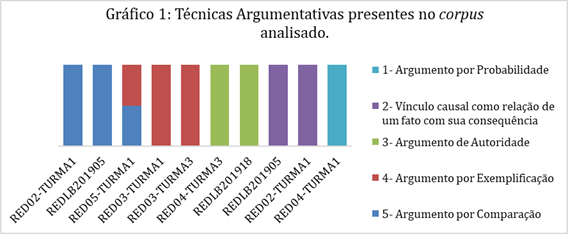
\includegraphics[width=0.85\textwidth]{fig2-33162.png}
 \caption{Gráfico 1: Tendências Argumentativas presentes no \emph{corpus} analisado.}
 \label{fig2}
 \source{Elaborado pelos autores.}
\end{figure}

Portanto, com este estudo foi possível observar que utilizar os recursos tecnológicos do Portal PROENEM (Unilab), como forma de estudo individual ou coletivo, proporciona um ensino-aprendizagem de maneira eficaz para a construção do conhecimento e da utilização adequada das estratégias argumentativas em textos estilo ENEM. Os recursos tecnológicos do Portal, como vimos, podem contribuir de maneira significativa para a escrita de estudantes que almejam cursar um ensino superior, mostrando-se como mecanismo eficaz no exercício de uma interatividade importante para o processo de ensino-aprendizagem dos pré-universitários.


\printbibliography\label{sec-bib}
% if the text is not in Portuguese, it might be necessary to use the code below instead to print the correct ABNT abbreviations [s.n.], [s.l.] 
%\begin{portuguese}
%\printbibliography[title={Bibliography}]
%\end{portuguese}


%full list: conceptualization,datacuration,formalanalysis,funding,investigation,methodology,projadm,resources,software,supervision,validation,visualization,writing,review
\begin{contributors}[sec-contributors]
\authorcontribution{Adriely da Silva Clemente}[conceptualization,datacuration,formalanalysis,investigation,writing,review]
\authorcontribution{Leonardo Chaves Ferreira}[conceptualization,investigation,writing,review]
\authorcontribution{José Olavo da Silva Garantizado Júnior}[projadm,supervision,validation,writing]
\end{contributors}


\end{document}
